\RequirePackage[l2tabu, orthodox]{nag}
\documentclass[10pt]{book}

% Language support
\usepackage[spanish, english]{babel}


% Thesis format
\usepackage[paperheight=24cm, paperwidth=17cm]{geometry}

% Graphics support
\usepackage{graphicx}
\graphicspath{{figures/}}

% Useful math features
\usepackage{amssymb}
\usepackage{amsmath}
\usepackage{bm}

% Alter geometry of the page headers:
\usepackage{fancyhdr} 

% Fancy tables
\usepackage{booktabs}

%Citations are numbered, sorted and consequtive lists compressed:
\usepackage[numbers, compress, sort]{natbib}

% Allow appendices in chapters:
\usepackage[toc]{appendix}

% Sans serif for section names:
\usepackage{sectsty}
\allsectionsfont{\sffamily}
\chapterfont{\LARGE \sffamily}

% Setting header height:
\headheight 14pt

% Setting text size:
\setlength{\textwidth}{12.3cm}
\setlength{\textheight}{18.5cm}

% Setting margins:
\setlength{\oddsidemargin}{-1in}
\setlength{\evensidemargin}{-1in}
\setlength{\topmargin}{-1in}
\addtolength{\oddsidemargin}{2.5cm}
\addtolength{\evensidemargin}{2.2cm}
\addtolength{\topmargin}{1.8cm}

% Parameters for fancy headers:
\pagestyle{fancyplain}
\renewcommand{\chaptermark}[1]{\markboth{\chaptername\ \thechapter.\ #1}{}}
\renewcommand{\sectionmark}[1]{\markright{\thesection\ #1}}
\lhead[\fancyplain{}{\thepage}]{\fancyplain{}{\rightmark}}
\rhead[\fancyplain{}{\leftmark}]{\fancyplain{}{\thepage}}
\cfoot{}

% Alter some LaTeX defaults for better treatment of figures.  Taken from
% http://mintaka.sdsu.edu/GF/bibliog/latex/floats.html
\renewcommand{\topfraction}{0.9}    % max fraction of floats at top
\renewcommand{\bottomfraction}{0.8} % max fraction of floats at bottom
\renewcommand{\textfraction}{0.1}   % allow minimal text w. figs

% Hyphenation:
\hyphenation{Ber-cea-nu Mar-chet-ti Ca-ru-sot-to}

% Abbreviations:
\newcommand*{\Lca}{\mathcal{L}}


\newcommand*{\la}{\langle}
\newcommand*{\ra}{\rangle}
\newcommand*{\abs}[1]{\vert #1 \vert}
\newcommand*{\bra}[1]{\langle #1 \vert}
\newcommand*{\ket}[1]{\vert #1 \rangle}
\newcommand*{\braket}[2]{\langle #1 \vert #2 \rangle}

\newcommand*{\zb}{\bar{z}}
\newcommand*{\e}{\epsilon}

\newcommand*{\rv}{\bm{r}}
\newcommand*{\kv}{\bm{k}}
\newcommand*{\kop}{\hat{\bm{k}}}


% \colvec{a}{b}
\newcommand*\colvec[2]{
  \begin{pmatrix}
    #1\\
    #2
  \end{pmatrix}
}

% \mat{a}{b}{c}{d}
\newcommand*{\mat}[4]{
  \begin{pmatrix}
    #1 & #2\\
    #3 & #4
  \end{pmatrix}
}

\newcommand*{\etal}{\emph{et al.}}

\DeclareMathOperator{\real}{Re}
\DeclareMathOperator{\imag}{Im}

\DeclareMathOperator{\Ry}{\mathcal{R}y}

\newcommand{\noo}[1]{: \negthinspace {#1} \negthinspace :}


\begin{document}
\frontmatter

\thispagestyle{empty}

\begin{center}
{\Huge  Scattering and topological properties of \\ driven-dissipative quantum fluids\\}
\vspace{5.4cm}
{\large{TESIS DOCTORAL}}\\
\vspace{2.6cm}
{ \textsc{memoria presentada para optar al grado de \\ Doctor en Ciencias F\'{i}sicas\\
Universidad Aut\'{o}noma de Madrid\\
Departamento de F\'{i}sica Te\'{o}rica de la Materia Condensada\\
Programa de Doctorado\\
F\'{i}sica de la Materia Condensada y Nanotecnolog\'{i}a\\
day-of-week day month year\\ %TODO: update when defense date is known
$\,$\\$\,$\\por\\$\,$\\$\,$\\}
{\LARGE{Andrei Ciprian Berceanu}}\\$\,$ \\\textsc{nacido en Bucarest, Ruman\'{i}a en 1983}}
\end{center}
\newpage

\thispagestyle{empty}
\noindent {\large\bfseries Comisi\'{o}n:}\\[2ex]
  \parbox[t]{2.8cm}{Director:\\
                  Tribunal:
}~\parbox[t]{9cm}{Prof.\ dr.\ F.\ M.\ Marchetti (UAM) \\
Prof.\ dr.\ C.\ Tejedor (UAM) \\
Prof.\ dr.\ L.\ Vi\~{n}a (UAM) \\
Dr.\ A.\ Amo (CNRS, France) \\
Dr.\ J.\ J.\ Garc\'{\i}a-Ripoll (CSIC) \\
Dr.\ T.\ Ozawa (Universit\`{a} di Trento, Italy)
}

% TODO: check members of the committee

\vfill


\noindent
\begin{otherlanguage}{spanish}
El autor agradece el apoyo financiero de FP7 ITN ``Clermont4'' y
de la European Science Foundation (ESF) a trav\'{e}s de POLATOM Grant 4914.
\end{otherlanguage}
\vspace{\baselineskip}


\noindent
The author acknowledges financial support from FP7 ITN ``Clermont4'' and
from the European Science Foundation (ESF) through POLATOM Grant 4914.
\vspace{\baselineskip}


\begin{center}
\includegraphics[width=30mm]{uam_logo}  
\end{center}


\newpage

\thispagestyle{empty}

\phantom{text}

\vspace{2cm}

\begin{flushright}
  {\em Bunicilor mei.}
\end{flushright}

\newpage

\thispagestyle{empty}

%%% Local Variables:
%%% mode: latex
%%% TeX-master: "thesis_berceanu"
%%% End:



\tableofcontents
\mainmatter

\chapter{Introduction}

% TODO: insert chapter descriptions (see akhmerov)
% TODO: create abbreviations list
% GP: Gross-Pitaevskii
% TODO: mention \hbar = 1


\section{Preliminaries}
\label{sec:preliminary}

\subsection{Linear response theory}
\label{subsec:linear-response}

Let $\phi_0(\rv)$ be the steady state solution to the
GP equation in the time-independent trapping potential $U_0(\rv)$
%
\begin{equation}\label{eq:GP-atoms}
  H_{\text{GP}} \phi_0 = 0
\end{equation}
% 
with the GP Hamiltonian defined as\footnote{This section follows
  loosely the formalism presented in Ref.~\cite{9783540410478}.}
%
\begin{equation}\label{eq:GP-ham}
  H_{\text{GP}} \equiv -\frac{\nabla^2}{2m} + U_0 + gN_0\abs{\phi_0}^2 - \mu
\end{equation}
% 

This Hamiltonian describes a bosonic condensate of $N_0$ particles with
contact interactions quantified by $g$, and chemical potential $\mu$.

Now consider adding a small time-dependent perturbation on top of the
trap, giving $U(\rv,t)=U_0(\rv) + \delta U(\rv,t)$. We are interested
in the response of the condensate to this perturbation.  For weak
perturbations, we can perform a linearization of the GP equation
Eq.~\eqref{eq:GP-atoms} around the stationary solution $\phi_0$. This
approach is known in the literature as the ``linear response''
formalism.

The condensate wavefunction $\phi(\rv,t)$ evolves according to
%
\begin{equation}\label{eq:GP-atoms-evolution}
  i\partial_t \phi = \left[-\frac{\nabla^2}{2m} + U + gN_0 \abs{\phi}^2 - \mu\right] \phi
\end{equation}
% 
We assume a small deviation of the wavefunction from its initial
steady state
%
\begin{equation}\label{eq:ansatz-atoms}
  \phi(\rv,t) = \phi_0(\rv) + \delta\phi(\rv,t)
\end{equation}
% 
such that we can expand Eq.~\eqref{eq:GP-atoms-evolution} and keep only linear terms in $\delta\phi$ and $\delta U$. We get
%
\begin{equation}\label{eq:GP-atoms-lin}
  i\partial_t\delta\phi =  \left[-\frac{\nabla^2}{2m} + U_0-\mu\right]
  \delta\phi + 2 g N_0 \phi_0^{\star}\phi_0\delta\phi + gN_0\phi_0^2\delta\phi^{\star}
  +\delta U\phi_0
\end{equation}
% 
Note that Eq.~\eqref{eq:GP-atoms-lin} is not strictly linear due to
the coupling of $\delta\phi$ to $\delta\phi^{\star}$. To restore
linearity, we consider the functions $\delta\phi$ and
$\delta\phi^{\star}$ as being independent and write the linear system
%
\begin{equation}\label{eq:GP-atoms-system}
  i \partial_t \colvec{\delta\phi(\rv,t)}{\delta\phi^{\star}(\rv,t)}
  = \Lca_{GP} \colvec{\delta\phi(\rv,t)}{\delta\phi^{\star}(\rv,t)}
  + \colvec{S(\rv,t)}{-S^{\star}(\rv,t)}
\end{equation}
% 
where we have introduced the linear operator
%
\begin{equation}\label{eq:LGP}
  \Lca_{\text{GP}} = \mat{H_{\text{GP}}+gN_0\abs{\phi_0}^2}{g N_0 \phi_0^2}{-g N_0 \phi_0^{\star 2}}{-\left[H_{\text{GP}}+gN_0\abs{\phi_0}^2\right]^{\star}}
\end{equation}
% 
and the source term $S(\rv,t)=\delta U(\rv,t)\phi_0(\rv)$.  Note that
$\Lca_{\text{GP}}$ is not a Hermitian operator! The presence of the minus
sign in the second line is due to the fact that the particles obey
Bose statistics, as this is not present in the BCS theory.

The standard method of determining the time evolution of $\delta\phi$
is to expand it in the basis formed by the eigenvectors of
$\Lca_{\text{GP}}$.

There is a subtlety involved here, however, as in the general case
$\Lca_{\text{GP}}$ is not diagonalizable. It usually has too few
eigenvectors to span the whole functional space\footnote{We are
  referring to the $L^2 \times L^2$ space, with $L^2$ being the space
  of square-integrable complex functions.}.

The solution to this problem, detailed in Ref.~\cite{Castin_1998},
is to work in the subspace orthogonal to $\ket{\phi_0}$. It can be
shown that the component of the solution along $\ket{\phi_0}$ only
results in a change of phase of the total condensate wavefunction. For
the problems of interest in the rest of this manuscript, however, the
dimension of the space parallel to $\ket{\phi_0}$ that we must project
out is of order 1.

We now consider the eigenvalue equation for the operator $\Lca_{\text{GP}}$
%
\begin{equation}\label{eq:L-eigen}
  \Lca_{\text{GP}} \ket{\psi_k^R} = \epsilon_k \ket{\psi_k^R}
\end{equation}
% 
with $\ket{\psi_k^R}$ being the right eigenvector and $\epsilon_k$ its
corresponding eigenvalue
%
\begin{equation}\label{eq:psi-R}
  \ket{\psi_k^R} = \colvec{\ket{u_k}}{\ket{v_k}}
\end{equation}
% 
Similarly, we also introduce the left eigenvector, obeying
$\Lca_{\text{GP}}^{\dagger} \ket{\psi_k^L} = \epsilon_k^{\star} \ket{\psi_k^L}$,
and the orthonormality condition
$\braket{\psi_k^L}{\psi_q^R} = \delta_{k,q}$. 

Notice that $\Lca_{\text{GP}}$ and $\Lca_{\text{GP}}^{\dagger}$ are
connected by the unitary transformation\footnote{Note that this holds
  as long as the Hamiltonian $H_{\text{GP}}$ only contains real
  terms.}
%
\begin{equation}\label{eq:symmetry-1}
  \eta \Lca_{\text{GP}} \eta^{\dagger} = \Lca_{\text{GP}}^{\dagger}
\end{equation}
% 
where $\eta = \sigma_3 = \mat{1}{0}{0}{-1}$ is the third Pauli
matrix. We say that $\Lca_{\text{GP}}$ is $\eta$-Hermitian, meaning
that one can define a new scalar product
$\braket{\cdot}{\cdot}_{\eta} \equiv \braket{\cdot}{\eta \cdot}$ with a
different signature, such that
$\braket{\cdot}{\Lca_{\text{GP}} \cdot}_{\eta} =
\braket{\Lca_{\text{GP}} \cdot}{\cdot}_{\eta}$. The operator $\eta$ is
usually called the metric operator, and, not suprisingly in our case,
it is the same as the one of the scalar Klein-Gordon equation. A
pseudo-Hermitian operator usually also posesses antilinear symmetries,
and as we will see below this is also the case for
$\Lca_{\text{GP}}$. Interestingly, for operators with a real spectrum,
it can be shown that one can define another metric $\eta_+$, which
guarantees a positive-definite inner product, or, in other words,
$\braket{\psi}{\psi}_{\eta_+} > 0$ (provided $\psi \neq 0$ of
course). This can be used to formulate a probabilistic quantum theory
for the new wave-functions $\psi^R$ and $\psi^L$. For the general
theory and properties of pseudo-Hermitian operators, we point the
interested reader to Ref.~\cite{MOSTAFAZADEH_2010}.


Using Eq.~\eqref{eq:symmetry-1}, we get the general form of the left
eigen-vectors as
%
\begin{equation}\label{eq:psi-L}
  \bra{\psi_k^L} = {\cal N}_k \left( \bra{u_k},\, -\bra{v_k} \right)
\end{equation}
% 
with ${\cal N}_k$ a normalization factor.  We can chose
${\cal N}_k = \pm 1$ and group the eigenvalues of $\Lca_{\text{GP}}$
into 3 families, according to the quantity
%
\begin{equation}\label{eq:norms}
  n_k = \braket{u_k}{u_k} - \braket{v_k}{v_k}
\end{equation}
% 
We therefore have: the ``$+$'' family, corresponding to $n_k=+1$, the
``$-$'' family, such that $n_k=-1$ and the ``$0$'' family, with
$n_k=0$.

% In the absence of the added weak perturbation, the time evolution of
% mode $k$ is given by $\exp(-i\epsilon_k t)$, from which we get the
% dynamical stability condition $\imag{(\epsilon_k)} \leq 0$ for all
% $k$. Dynamical stability is important because it insures that small
% perturbations will not induce the condensate wavefunction to evolve
% far from its steady state value.

We are now ready to write the completeness relation
%
\begin{equation}\label{eq:completeness}
  \sum_k \ket{\psi_k^R} \bra{\psi_k^L} = \mathbb{I}
\end{equation}
% 
Using Eq.~\eqref{eq:completeness}, we can decompose any column vector
as\footnote{The modes in the ``$0$'' family do not appear in this
  expansion as their components live in the space orthogonal to the one
  of our solution.}
%
\begin{multline}\label{eq:decomposition}
  \colvec{\ket{l_1}}{\ket{l_2}} = \sum_{k \in ``+" \mbox{\scriptsize family}} \left[\braket{u_k}{l_1} - \braket{v_k}{l_2}\right]\colvec{\ket{u_k}}{\ket{v_k}}\\
  + \sum_{k \in ``-" \mbox{\scriptsize family}} \left[\braket{v_k}{l_2} - \braket{u_k}{l_1}\right]\colvec{\ket{u_k}}{\ket{v_k}}
\end{multline}
% 
There is now a further symmetry of $\Lca_{\text{GP}}$ that we can
exploit in our problem, a sort of time-reversal ``spin''-flip (or
particle-hole) symmetry, namely
%
\begin{equation}\label{eq:symmetry-2}
   \Theta \Lca_{\text{GP}} \Theta^{\dagger} = -\Lca_{\text{GP}}
\end{equation}
%
where $\Theta = \sigma_1 \cal{K}$, with $\sigma_1 = \mat{0}{1}{1}{0}$
the first Pauli matrix and $\cal{K}$ the complex conjugation
antilinear operator.

This results in a duality between the ``$+$'' family with eigenvectors
$(u_k, v_k)$ and energy $\epsilon_k$ and the ``$-$'' family with
eigenvectors $(v_{-k}^{\star}, u_{-k}^{\star})$ and energy
$-\epsilon_{-k}^{\star}$.

We can now finally project Eq.~\eqref{eq:GP-atoms-system} onto the
eigenvectors of $\Lca_{\text{GP}}$. Using the above-mentioned duality and
Eq.~\eqref{eq:decomposition}, we get
%
\begin{equation}\label{eq:phi-column-expansion}
  \colvec{\delta\phi(\rv,t)}{\delta\phi^{\star}(\rv,t)} = \sum_{k \in ``+" \mbox{\scriptsize family}}
  b_k(t) \colvec{u_k(\rv)}{v_k(\rv)}
  + b_{-k}^{\star}(t) \colvec{v_{-k}^{\star}(\rv)}{u_{-k}^{\star}(\rv)}
\end{equation}
% 
with the complex amplitudes $b_k$ satisfying 
%
\begin{equation}\label{eq:amplitudes-bk}
  i \frac{d}{dt}b_k(t) = \epsilon_k b_k(t) + s_k(t)
\end{equation}
% 
where we introduced
%
\begin{equation}\label{eq:amplitudes-sk}
  s_k(t) = \left( \bra{u_k} ,\, -\bra{v_k} \right) \colvec{\ket{S(t)}}{-\ket{S^{\star}(t)}}
\end{equation}
% 

\subsection{Cherenkov emission}
\label{subsec:cherenkov}

We now turn to applying the formalism developed in
Sec.~\ref{subsec:linear-response} to a concrete physical example,
inspired by Ref.~\cite{Carusotto_2006}. Consider a 2-dimensional
Bose-Einstein atomic condensate in a state with well-defined momentum,
described by the plane wave
$\psi_0 \exp \left( i \bm{k_0} \rv - \omega_0 t \right)$. Using our
previous notation, this corresponds to
%
\begin{equation}\label{eq:atom-initial}
  \phi_0(\rv) = \psi_0 \exp \left( i \bm{k_0} \rv \right)
\end{equation}
% 
and a chemical potential $\mu = \omega_0$. Since we have no trap,
$U_0(\rv)=0$, and Eq.~\eqref{eq:GP-atoms} reduces to
%
\begin{equation}\label{eq:atom-MF}
  \omega_0 - \left( \frac{k_0^2}{2m} + g \rho_0 \right) = 0
\end{equation}
% 
where we have introduced the condensate density
$\rho_0 \equiv N_0 \abs{\psi_0}^2$.  

We now intoduce a weak perturbation in the form of a localized defect
potential $\delta U(\rv, t) = V_d(\rv)$, which can represent for
instance a laser spot depleting a small area of the condensate.

Using Eq.~\eqref{eq:atom-MF}, the GP Hamiltonian becomes
$H_{\text{GP}} = -\frac{\nabla^2}{2m} - \frac{k_0^2}{2m}$ and the
source term
$S(\rv) = \psi_0 V_d(\rv) \exp \left( i \bm{k_0} \rv \right)$. We now
get the linear operator for our problem in the form
%
\begin{equation}\label{eq:ourL}
  \Lca = \mat{-\frac{\nabla^2}{2m} - \frac{k_0^2}{2m} + g\rho_0}{g N_0 \psi_0^2 \exp \left( 2 i \bm{k_0} \rv \right)}{- g N_0 \psi_0^{\star 2} \exp \left( - 2 i \bm{k_0} \rv \right)}{-\left[ -\frac{\nabla^2}{2m} - \frac{k_0^2}{2m} + g\rho_0 \right]}
\end{equation}
% 
Notice that, due to the presence of the off-diagonal exponential
terms, $\Lca$ does not commute with the momentum operator, which is
the generator of the spatial translation group. Luckily, however, we
can restore translational invariance by a simple unitary
transformation, as shown below.

First, a brief reminder of basic quantum mechanics. Using the standard
commutation relations, one can show that, for a constant wavevector
$\bm{k_0}$, the unitary operator\footnote{The hat symbol denotes
  operators in the relevant Hilbert space.}
%
\begin{equation}\label{eq:trans-oper}
  \hat{T}(\bm{k_0}) = \exp \left( -i \bm{k_0} \hat{\rv} \right)
\end{equation}
% 
performs a translation in momentum space,
$\hat{T}(\bm{k_0}) \ket{\bm{k}} = \ket{\bm{k} - \bm{k_0}}$, with the
ket $\ket{\bm{k}}$ representing a single particle state with
wavevector $\bm{k}$ such that
$\hat{\bm{k}} \ket{\bm{k}} = \bm{k} \ket{\bm{k}}$. Using the
definitions above, one can easily obtain the commutator
%
\begin{equation}\label{eq:trans-commutator}
  \left[ \hat{\bm{k}},\, \hat{T}(\bm{k_0}) \right] = -\bm{k_0}\hat{T}(\bm{k_0}) 
\end{equation}
% 
This allows us to rewrite the following expressions
\begin{align}\label{eq:products}
  \begin{split}
    \hat{T}^{\dagger}(\bm{k_0})\hat{\bm{k}}\hat{T}(\bm{k_0})& = \hat{\bm{k}} - \bm{k_0}\hat{\mathbb{I}}\\
    \hat{T}(\bm{k_0})\hat{\bm{k}}\hat{T}^{\dagger}(\bm{k_0})& = \hat{\bm{k}} + \bm{k_0}\hat{\mathbb{I}}  
  \end{split}
\end{align}

We now recognize the two exponentials in Eq.~\eqref{eq:ourL} as being
the real-space representation of $\hat{T}^2(\bm{k_0})$ and its
hermitian conjugate. This motivates us to define the following unitary
operator
%
\begin{equation}\label{eq:ucal}
  \hat{{\cal T}}(\bm{k_0}) = \mat{\hat{T}(\bm{k_0})}{0}{0}{\hat{T}^{\dagger}(\bm{k_0})}
\end{equation}
% 
such that a unitary transformation of our operator $\Lca$ now restores translational
symmetry. Indeed, one can see that
%
\begin{equation}\label{eq:translated-L}
  \hat{{\cal T}} \hat{\Lca} \hat{{\cal T}}^{\dagger} = \mat{\frac{\left(\kop + \bm{k_0}\right)^2}{2m} - \frac{k_0^2}{2m} + g\rho_0}{g N_0 \psi_0^2}{- g N_0 \psi_0^{\star 2}}{-\left[\frac{\left(\kop - \bm{k_0}\right)^2}{2m} - \frac{k_0^2}{2m} + g\rho_0 \right]}
\end{equation}
% 
where we have make use of Eqs.~\eqref{eq:products} and we have written
$\hat{\Lca}$ in a base-independent representation.  In the subspace of
momentum eigenstates $\ket{\kv}$, we can write the (right-)eigenvalue
equation corresponding to Eq.~\eqref{eq:translated-L} as
%
\begin{equation}\label{eq:right-eigen}
  \Lca_{\text{GP}} [k] \colvec{U_\sigma(k)}{V_\sigma(k)} = \epsilon_\sigma(k) \colvec{U_\sigma(k)}{V_\sigma(k)}
\end{equation}
% 
where we have recovered the matrix representation of
Eq.~\eqref{eq:LGP}, and introduced the notation
$\omega_\sigma(\kv) = \bm{v}_0 \kv + \epsilon_\sigma(k)$. Here
$\sigma = \pm$ labels the 2 different eigenmodes and we defined
$\bm{v}_0 \equiv \frac{\kv_0}{m}$ as the speed of the condensate.

Notice that the $k=0$ mode has only one eigenvector. However, one can
safely exclude it as this mode does not imply energy or momentum
transport. Excluding the $k = 0$ point, one can then solve
Eq.~\eqref{eq:right-eigen} and obtain the celebrated Bogoliubov
excitation spectrum
%
\begin{equation}\label{eq:bogoliubov}
  \epsilon_\sigma(k) = \sigma \left[\frac{k^2}{2m}\left(\frac{k^2}{2m} + 2 g \rho_0 \right) \right]^{\frac{1}{2}}
\end{equation}
% 
with $\sigma = \pm$. Notice that the complex amplitudes $U_\sigma(k)$,
$V_\sigma(k)$ only depend on the absolute value of $\kv$, while the
(real) spectrum of Eq.~\eqref{eq:translated-L}, $\omega_\sigma(\kv)$
is the Bogoliubov spectrum with an additional Galilean boost
$\bm{v}_0 \kv$.

As can be seen from Eq.~\eqref{eq:symmetry-2}, the 2 eigen-families
$\sigma$ and $-\sigma$ are linked by a duality, stemming from the
$\cal{P} \cal{T}$ symmetry\footnote{This can be actually formally
  proven after defining the parity and time-reversal operators
  corresponding to our problem. For details, see
  Ref.~\cite{MOSTAFAZADEH_2010}.} of the Bogoliubov operator $\Lca$.
We therefore drop the subscript and make the convention that
$\left( U,\, V \right) \equiv \left( U_{+},\, V_{+}
\right)$. Furthermore, making use of Eq.~\eqref{eq:symmetry-1}, we can
act with $\sigma_3$ on the eigenstates of $\Lca_{\text{GP}}$ to obtain
the ones of $\Lca_{\text{GP}}^{\dagger}$. 

This finally leads us to a biorthonormal basis
$\left\{ \ket{\psi_\sigma^R(\kv)},\, \ket{\psi_\sigma^L(\kv)} \right\}$
with 4 basis vectors
%
\begin{equation}\label{eq:biorthobasis}
  \left\{ \colvec{U(k)}{V(k)}, \colvec{V^{\star}(k)}{U^{\star}(k)}, \colvec{U(k)}{-V(k)}, \colvec{-V^{\star}(k)}{U^{\star}(k)} \right\} \bigotimes \ket{\kv}
\end{equation}
% 
which fulfills the orthonormality condition
%
\begin{equation}\label{eq:binormality}
  \braket{\psi_{\sigma^{\prime}}^L(\kv^{\prime})}{\psi_\sigma^R(\kv)} = \delta_{\sigma,\sigma^{\prime}} \delta^2(\kv - \kv^{\prime})
\end{equation}
% 
provided of course that we normalize in such a way that
$\abs{U(k)}^2 - \abs{V(k)}^2 = 1$, and the completeness relation
%
\begin{equation}\label{eq:bicompleteness}
  \sum_{\sigma = \pm} \int d^2 \kv \; \ket{\psi_\sigma^R(\kv)}\bra{\psi_\sigma^L(\kv)} = 1
\end{equation}
% 
In this basis, the spectral decomposition of
Eq.~\eqref{eq:translated-L} is of the diagonal form
%
\begin{equation}\label{eq:bidecomposition}
  \hat{{\cal T}} \hat{\Lca} \hat{{\cal T}}^{\dagger} = \sum_{\sigma = \pm} \int d^2 \kv \; \omega_\sigma(\kv) \ket{\psi_\sigma^R(\kv)}\bra{\psi_\sigma^L(\kv)}
\end{equation}
% 
The concrete form of $\Lca_{\text{GP}}[k]$, coupled with the
normalization condition Eq.~\eqref{eq:norms}, determines the
eigenvectors of the ``+'' family up to a phase factor. Indeed, one can
choose $\abs{U(k)} \pm \abs{V(k)} = f(k)^{\pm\frac{1}{4}}$, with 
%
\begin{equation}\label{eq:norms}
  f(k) = \frac{\frac{k^2}{2m}}{\frac{k^2}{2m} + 2g\rho_0}
\end{equation}
% 
It is now a trivial matter to solve the linearized evolution equation
Eq.~\eqref{eq:GP-atoms-system} for our problem. In particular, for a
localized static defect potential $V_d(\rv) = g_V \delta^2(\rv)$,

\section{Microcavity exciton-polaritons}
\label{sec:polaritons}


Consider the following (simplified) physical system. We have a bunch
of photons confined within the metalic mirrors of an optical cavity
which also contains a 2D semiconductor quantum well (QW), as shown in
Fig.~\ref{fig:cavity-polaritons}. The photons continuously create
electron-hole pairs, which go by the name of excitons, within the
QW. The excitons in turn recombine, emiting photons, which every so
often escape through the imperfect cavity mirrors. If one uses a
continuous wave laser to replenish the lost photons, a steady state
can eventually be reached where the pumping balances the losses. The
system is however in a driven-dissipative state, out of thermal
equilibrium.

Exactly describing the system of electrons, holes and photons, taking
into account their Coulomb interaction and the disorder created by
defects inside the QW, as well as imperfections in the mirrors would
not allow for much physical insight into this problem. We therefore
use a series of approximations in order to construct an effective
Hamiltonian description of the system.
%
\begin{figure}[tb]\centering
  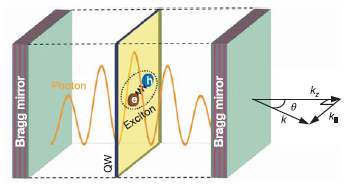
\includegraphics[width=.8\linewidth]{cavity}
  \caption{
    % 
    Pictorial representation of microcavity polaritons, as electron-hole pairs (excitons) inside a semiconductor quantum well, 
coupled with the photons trapped by the dielectric Bragg mirrors of the cavity. To excite the polariton mode with wave-vector $\kv$, a beam with incidence angle $\theta$ has to hit the microcavity, such that $k c = \omega \sin\theta$, with $\omega$ being the beam frequency.
From Ref.~\cite{Kasprzak_2006}.
    % 
}\label{fig:cavity-polaritons}
\end{figure}
% 
We start by writing down the kinetic energy of the photons
%
\begin{equation}\label{eq:cavity-energy}
  H_{C} = \sum_{\kv} E_C(k) a_{\kv}^{\dagger} a_{\kv}
\end{equation}
% 
where we've made use of the translational symmetry of the problem in
the $(x,y)$ plane and labeled the bosonic creation (annihilation)
operators $a_{\kv}^{\dagger}$ ($a_{\kv}$) by the in-plane momentum
$\kv$. The confinement along the $z$ direction leads to quantization
of the photon momentum $k_z = \frac{2 \pi N}{l_z}$, with
$N = 1,2,\dots$ indexing the longitudinal modes ($N=5$ in
Fig.~\ref{fig:cavity-polaritons}) and $l_z$ being the cavity width,
i.e. the distance between the mirrors. The cavity photon dispersion
for each of these modes is therefore $E_C(k) = v \sqrt{k^2 + k_z^2}$,
with $v$ the speed of light in the semiconductor. Expanding the square
root for $k \ll k_z$, one has
$E_C(k) \approx E_C(0) + \frac{k^2}{2m_{C}}$. We see that
cavity photons, as opposed to free-space photons, have a quadratic
dispersion with an effective mass
$m_{C} = \frac{E_C(0)}{v^2}$. For typical cavities used in
experiments, $m_{C}$ is of the order of $10^{-5}$ (free)
electron masses $m_e^0$.

We now turn our attention to the semiconductor QW. For simplicity,
consider a spin-polarized direct bandgap semiconductor such as GaAs,
so that we can neglect additional spin degrees of freedom. We further
assume that the dispersions of single particle states in the
conduction and valence bands have the quadratic form
$\varepsilon^c_{k} = \varepsilon_g/2 + k^2/(2m_e)$ and
$\varepsilon^v_{k} = - \varepsilon_g/2 - k^2/(2m_h)$, with
$\varepsilon_g$ the semiconductor bandgap and $m_e$ and $m_h$ the
effective masses for electrons and (heavy) holes. Excitons have a
typical extension $\lambda_X = \frac{\epsilon}{2\mu e^2}$ called the
(2D) exciton Bohr radius, with $\epsilon$ the static dielectric
constant, $e$ the electron charge and $\mu^{-1} = m_e^{-1} + m_h^{-1}$
their reduced mass. Their binding energy is called the exciton
Rydberg, defined as $\Ry_X = \frac{e^2}{\epsilon \lambda_X}$.

Defining $c_{\kv}^{\dagger}$ and $v_{\kv}$ as the operators creating
an electron in the empty conduction band, respectively a hole in the
filled valence band, we can write the electronic hamiltonian as
%
\begin{equation}\label{eq:coulomb-hamiltonian}
  H_{\text{el}} = \sum_{\kv} \left( \varepsilon^c_k c_{\kv}^{\dagger} c_{\kv} + \varepsilon^v_k v_{\kv}^{\dagger} v_{\kv} \right) + \frac{1}{2}\sum_{\bm{q}} V_q \left( \rho^e_{\bm{q}} \rho^e_{-\bm{q}} + \rho^h_{\bm{q}} \rho^h_{-\bm{q}} -2 \rho^e_{\bm{q}} \rho^h_{-\bm{q}}\right)
\end{equation}
% 
Here we have introduced the electron and hole densities,
$\rho^e_{\bm{q}} = \sum_{\kv} c_{\kv + \bm{q}}^{\dagger} c_{\kv}$ and
$\rho^h_{\bm{q}} = \sum_{\kv} v_{\kv} v_{\kv + \bm{q}}^{\dagger}$. The
matrix element of the Coulomb potential
$V_q = \frac{e^2}{2 \epsilon A q}$ depends on cavity quantization area
$A$, but this dependence drops out when passing from discrete sums
over states to intragrals over $\kv$.

Finally, the last ingredient of our microscopic description concerns
the interaction between electrons and photons. Making use of the
dipole and rotating wave approximations, we have
%
\begin{equation}\label{eq:dipolar-inter}
  H_{\text{dipole}} = \sum_{\kv, \bm{q}} G(q) \left( a_{\bm{q}}^{\dagger} v_{\kv + \bm{q}}^{\dagger} c_{\kv} + \text{H.c.}\right)
\end{equation}
% 
with the strength
$G(q) = e \mu_{\text{cv}}\sqrt{\frac{E_C(q)}{2\epsilon A l_z}}$
written in the dipole gauge, where $\mu_{\text{cv}}$ is the inter-band
dipole matrix element.

We are interested in an approximate description of the problem where
we can consider the excitons as fundamental quasiparticle excitations
from the ground state of the semiconductor and treat the Coulomb term
in Eq.~\eqref{eq:coulomb-hamiltonian} as an effective exciton-exciton
interaction. We then couple the resulting excitons to light, and
obtain the so-called \textbf{weakly interacting boson model} for
polaritons. The name stems from the fact that, at moderate
electron-hole densities, one can assume excitons to behave esentially
as bosons, and describe them using the Bose creation and annihilation
operators $b_{\kv}^{\dagger}$ and $b_{\kv}$. Therefore, making an Usui
transformation and truncating the interaction terms at fourth order
results in the following three-part effective Hamiltonian
%
\begin{equation}\label{eq:total-ham}
  H_{\text{eff}} = H_0  + H_{\text{XX}} + H_{XC}^{\text{sat}}
\end{equation}
% 
where we have defined
\begin{align}
  H_0 & =\sum_{\kv}\left(a_{\kv}^{\dagger},\, b_{\kv}^{\dagger}\right)\mat{E_C(k)}{\Omega_R}{\Omega_R}{E_X(k)}\colvec{a_{\kv}}{b_{\kv}}\label{eq:polariton-ham}\\
  H_{\text{XX}} & =\frac{1}{2}\sum_{\kv,\kv^{\prime},\bm{q}}U_{\kv - \kv^{\prime},\bm{q}}b_{\kv + \bm{q}}^{\dagger}b_{\kv^{\prime} - \bm{q}}^{\dagger}b_{\kv^{\prime}}b_{\kv}\label{eq:interaction-ham}\\
  H_{XC}^{\text{sat}} & =-\frac{\Omega_R}{\rho_{\text{sat}}A}\sum_{\kv,\kv^{\prime},\bm{q}}\left(b_{\kv^{\prime}-\bm{q}}^{\dagger}b_{\kv + \bm{q}}^{\dagger}b_{\kv}a_{\kv^{\prime}} + \text{H.c.}\right)\label{eq:saturation-ham}
\end{align}
$H_0$ contains the kinetic energy of the excitons and cavity photons,
as well as their harmonic coupling, ie. the conversion of an exciton
to a cavity photon at the Rabi frequency $\Omega_R$, which depends on
the overlap between the wavefunctions of the exciton and photon and
$\mu_{\text{cv}}$. Eq.~\eqref{eq:polariton-ham} can be diagonalized by
means of a unitary transformation of the form
%
\begin{equation}\label{eq:hopfield-trans}
  \colvec{p_{\kv}}{u_{\kv}} = \mat{X_k}{C_k}{-C_k}{X_k} \colvec{b_{\kv}}{a_{\kv}}
\end{equation}
% 
The normal modes of $H_0$ are called \textbf{upper and lower polaritons} and
correspond to the Bose operators $u_{\kv}$ and $p_{\kv}$, with
eigen-energies
%
\begin{figure}[tb]\centering
  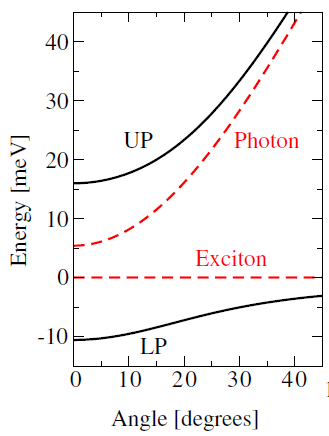
\includegraphics[width=.5\linewidth]{polariton_dispersion}
  \caption{
    % 
    Dispersion relation for the two polaritonic branches (UP, LP) as a function of emission angle $\theta$ of photons outside the cavity. This angle is connected to the momentum $k$ of polaritons inside the cavity by the relation $ck = E_{\text{LP}}(k) \sin \theta$. The exciton and cavity photon dispersions are depicted with dashed (red) lines. Notice the very sharp dispersion of the polaritons compared to excitons, due to the light mass of their photonic component.
From Ref.~\cite{Keeling_2007}.
    % 
}\label{fig:polariton-dispersion}
\end{figure}
% 
\begin{equation}\label{eq:polariton-dispersion}
  E_{\text{UP,LP}}(k) = \frac{1}{2}\left(E_C(k) + E_X(k)\right) \pm \frac{1}{2}\left[\left(E_C(k) - E_X(k)\right)^2 + 4 \Omega_R^2\right]^{1/2}
\end{equation}
% 
whereas the Hopfield coefficients appearing in Eq.~\eqref{eq:hopfield-trans} are
\begin{align}
  X_k & =\left[1 + \left(\frac{\Omega_R}{E_{\text{LP}}(k) - E_C(k)}\right)^2\right]^{-1/2}\label{eq:hopfield-X}\\
  C_k & =-\left[1 + \left(\frac{E_{\text{LP}}(k) - E_C(k)}{\Omega_R}\right)^2\right]^{-1/2}
\end{align}
The two branches of the polaritonic dispersion relation are shown in
Fig.~\ref{fig:polariton-dispersion}, together with the dispersions of
the cavity photons and excitons.

Note that the 1s-exciton energy can be approximated as
$E_X(k) = E_X(0) + \frac{k^2}{2M}$, with the exciton mass
$M = m_e + m_h$ of the order of the electron mass and
$E_X(0) = \varepsilon_g - \Ry_X$. Since, as we have already noted, $M$
is several orders of magnitude larger than the cavity photon mass
$m_{C}$, one can in practice neglect the momentum dependence
of the excitonic dispersion and consider it to be flat. Furthermore,
we can agree to measure energies starting from $E_X(0)$ and denote the
detuning between exciton and photon bands as
$\delta \equiv E_C(0) - E_X(0)$. For zero detuning ($\delta = 0$), the
splitting between the two polariton branches is $2\Omega_R$. In order
to tune $\delta$ in experiments, one tipically builds the cavity
mirrors with a wedge.

Also note that the spectrum in Fig.~\ref{fig:polariton-dispersion} is
represented as a function of the angle $\theta$ of emission of a
photon out of the cavity, as depicted in
Fig.~\ref{fig:cavity-polaritons}. Conservation of in-plane momentum
and photon frequency dictates that a laser beam coming in at an angle
$\theta$ and frequency $\omega$ resonantly excites a microcavity mode
with wave vector $k_{\parallel} = \frac{\omega}{c}\sin(\theta)$.

$H_{\text{XX}}$ quantifies the effective repulsive exciton-exciton
interaction, with a momentum-dependent strength
$U_{\kv - \kv^{\prime},\bm{q}}$ that can be calculated from the
Coulomb exchange term in the Born approximation. A further
approximation, for wave vectors much smaller than $\lambda_X^{-1}$, is
to reduce $U_{\kv - \kv^{\prime},\bm{q}}$ to a contact potential
$g_X \equiv \frac{1}{2} U_{\bm{0},\bm{0}} =
\frac{6e^2\lambda_X}{2A\epsilon}$. As a result $g_X$ physically
represents the interaction between two excitons in the same
single-particle momentum eigenstate $\ket{\kv}$.

Finally, the last term of Eq.~\eqref{eq:total-ham},
$H_{\text{XC}}^{\text{sat}}$, can be interpreted as a saturation
effect due to the Pauli exclusion principle underlying the fermionic
character of the excitons. The exciton saturation density
$\rho_{\text{sat}} = \frac{7}{16\pi\lambda_X^2}$ for the problems we
will be treating in the remainder of this manuscript can be considered
large enough to justify neglecting this anharmonic contribution to the
total Hamiltonian.

It is noteworthy to remark that Hamiltonian Eq.~\eqref{eq:total-ham}
does not include any disorder. We have already mentioned that there
are two distinct disorder classes in this problem. One is the
excitonic disorder, acting on length scales of around 10 nm, which
tipically affects the exciton oscillator strengths, but not the
spatial polaritonic density. This type of disorder stems from
variations in the QW thickness as well as alloy imperfections and is
typically not strong enough to dissociate excitons. Neglecting
excitonic disorder also implies that each localized exciton state
couples to precisely one extended photon state. The resulting
polaritons are then nothing but the superposition of these excitonic
and photonic states.

Photonic disorder, on the other hand, acts on lengthscales
$\ell_{C} = (m_{C}\Omega_R)^{-1/2}$ on the order of microns (see
Tab.~\ref{tab:GaAs-params}) and therefore can disrupt the polariton
density profile. It is normally caused by imperfections in the cavity
mirrors, which can act as scattering centers for the polaritons, and
can be included in the Hamiltonian as an additional external
potential. We will see some eloquent examples of polariton scattering
in the following chapters. Typical decay rates for excitons
($\gamma_X$) and cavity photons ($\gamma_C$) in GaAs-based
microcavities are also shown in Tab.~\ref{tab:GaAs-params}.

Last but not least, one should mention the validity limitations of the
weakly interacting boson model for polaritons. Its derivation, by
means of the Usui transformation, implies an expansion of the original
fermionic operators from Eq.~\eqref{eq:coulomb-hamiltonian} in powers
of bosonic operators, having as small parameter the number of excitons
per Bohr radius $\lambda_X$. Truncating the series results in an upper
bound on the exciton density of the order of $1/\lambda_X^2$. At
higher densities, an electron-hole plasma-like state is formed, with a
a qualitatively different behaviour.  We see that this model is
particularly useful for the case when the dominant interaction is the
Coulomb repulsion between the excitons.

For temperatures smaller than the Rabi splitting between the two
polariton branches, we can neglect the upper polaritons and project
Eq.~\eqref{eq:total-ham} on the basis of lower-polariton states
only. Employing the approximations we just mentioned, we obtain the
lower-polariton Hamiltonian
%
\begin{equation}\label{eq:LP-ham}
  H_{\text{LP}} = \sum_{\kv} E_{\text{LP}}(k) p_{\kv}^{\dagger} p_{\kv} + \sum_{\kv,\kv^{\prime},\bm{q}} V^{\text{eff}}_{\kv,\kv^{\prime},\bm{q}}\, p^{\dagger}_{\kv + \bm{q}} p^{\dagger}_{\kv^{\prime} - \bm{q}} p_{\kv} p_{\kv^{\prime}}
\end{equation}
% 
where the strength of the repulsive interaction between lower
polaritons now depends on in-plane momentum through the Hopfield
coefficients\footnote{The interaction strength $g_X$ can usually be
  rescaled to 1 by a simple transformation.}
%
\begin{equation}\label{eq:g-eff}
  V^{\text{eff}}_{\kv,\kv^{\prime},\bm{q}} = g_X X_{\kv + \bm{q}}X_{\kv^{\prime}}X_{\kv^{\prime} - \bm{q}}X_{\kv}
\end{equation}
% 
Physically, the quantities $\abs{X_k}^2$ and $\abs{C_k}^2$ are the
excitionic and photonic fractions of the lower lower polariton
mode. Their momentum dependence is not very pronounced, as for
$\delta = 0$, $X_k$ is between $1/\sqrt{2}$ and $1$ and if we are also
at normal incidence, meaning $\kv = 0$, than the light and matter
content of lower polaritons are each equal to $1/2$.

Consider now the low-temperature case, where the polaritons form a
BEC-like condensate in the momentum eigenstate $\ket{\kv}$. In this
case, since we have the macroscopic ocupation of a single particle
state, we can follow the standard Bogoliubov prescription and treat
the operator $p_{\kv}$ as a classical wavefunction, which we will
denote by $\psi_{\kv}$. The time-evolution of this classical object is
a Gross-Pitaevksii-like equation obtained from Heisenberg's equation
of motion
$i \partial_t \psi_{\kv}(t) = \left[\psi_{\kv}(t),\, H_{\text{LP}}\right]$.
Since polariton condensates are intrinsically out-of-equilibrium
systems, one also had to add additional terms in order to describe
pumping and losses. We therefore get a driven-dissipative mean-field
equation, which in momentum space reads
%
\begin{multline}\label{eq:mom-GPE}
  i\partial_t\psi_{\kv} = \left[E_{\text{LP}}(k) - \frac{i}{2} \gamma_k\right]\psi_{\kv} + \sum_{\kv_1,\kv_2} g_{\kv,\kv_1,\kv_2} \psi^{\star}_{\kv_1 + \kv_2 - \kv} \psi_{\kv_2} \psi_{\kv_1}\\
  + C_k f_p \exp{\left(-i \omega_pt\right)} \delta_{\kv,\kv_{p}}
\end{multline}
% 

%%%%%%

To get a more quantitative idea of the physics involved, it is worth
describing realistic samples typically used in state-of-the-art
experiments. Instead of simple metallic mirrors, such microcavities
are usually bound by a series of up to around 20 distributed Bragg
reflectors (DBRs), which are alternating dielectric layers of
thickness $\lambda/4$ and different refractive indices, achieving a
total reflectivity of over $99.9$\%. Multiple CdTe or GaAs QWs of
approximately $8~$nm thickness are placed inside the cavity of length
$l_z = 2\lambda \sim 1~\mu$m, at the antinodes (maxima) of the
photonic field, in order to maximize the coupling between excitons and
photons. Typical values of the relevant parameters for GaAs-based
microcavities are shown in Tab.~\ref{tab:GaAs-params}. As a sidenote,
one can see that for these values, the ratio between saturation and
Coulomb interaction
$\frac{\Omega_R}{g_X \rho_{\text{sat}}} \simeq 0.1$, hereby justifying
our assumption that we can neglect the anharmonic Hamiltonian
Eq.~\eqref{eq:saturation-ham}.
%
\begin{table}
  \centering
  \begin{tabular}{@{}ll@{}} \toprule
    QW & Cavity \\ \midrule
    $\epsilon \simeq 13$ &  $E_C(0) \simeq E_X(0) \simeq 1.53$~eV\\
    $m_e = 0.063m^0_e$    &  $\delta \in [-10,10]$~meV\\
    $m_h = 0.3m^0_e$      &  $m_{C} = 2.3\times 10^{-5} m^0_e$ \\
    $\lambda_X \simeq 7$~nm   & $\ell_{C} = 0.868~\mu$m\\
    $\Ry_X \simeq 17$~meV &  $\Omega_R \simeq 2.2$~meV \\
    $\gamma_X \sim \mu$eV &  $\gamma_C = 0.1$~meV \\ 
    $g_X \simeq 5\times10^{-3}$~meV($\mu$m)$^2$ &  $A = 10^4~\mu$m$^2$\\
    $\rho_{\text{sat}} \simeq 2842~$($\mu$m)$^{-2}$ &  $l_z \sim 1~\mu$m\\ \bottomrule
  \end{tabular}
  \caption{Typical parameters of a microcavity containing GaAs QWs, from Ref.~\cite{9783642241857}. Left column shows values concerning the QW while the right one refers to the microcavity.}
  \label{tab:GaAs-params}
\end{table}
%


%TODO: explanation of terms
%TODO: add defect potential
%TODO: real space driven-dissipative GPE
%TODO: different types of pumping
%TODO: mean-field equations, U(1)
%TODO: OPO
%TODO: add references
%TODO: anticrossing mention in disp fig, strong coupling
%TODO: polaritons = photons dressed by matter
%TODO: directly excited by laser and detected via reflection/transmission 




%%% Local Variables:
%%% mode: latex
%%% TeX-master: "../thesis_berceanu"
%%% End:

%%%%%%%%%%%%%%%%%%%%%%%%%%%%%%%%%%%
% Key                | Occurences | 
%--------------------+------------| 
% Cancellieri_2010   |         10 | 
% Wouters_2010 (*)   |          5 | 
% Astrakharchik_2004 |          5 | 
% Ciuti_2005         |          5 | 
% Amo_2009 (*)       |          4 | 
%%%%%%%%%%%%%%%%%%%%%%%%%%%%%%%%%%%


\chapter{Drag in a resonantly pumped polariton fluid}
\label{cha:drag}

\section{Introduction}
\label{sec:intro}

Out of equilibrium quantum fluids such as polaritons in semiconductor
microcavities are being the subject of an intensive study. Microcavity
polaritons, the quasiparticles resulting from the strong coupling of
cavity photons and quantum well excitons, have the prerogative of
being easy to both manipulate, via an external laser, and detect, via
the light escaping from the cavity~\cite{9780199228942}. In
particular, resonant excitation allows the accurate tuning of the
fluid properties, such as its density and current. However, the
polariton lifetime being finite establishes the system as
intrinsically out of equilibrium: An external pump is needed to
continuously replenish the cavity of polaritons, that quickly, on a
scale of tens of picoseconds, escape.

Recently, the superfluid properties of a resonantly pumped polariton
quantum fluid in the pump-only configuration --- i.e., where no other
states aside the pump one are occupied by, for example, parametric
scattering --- have been actively investigated both experimentally and
theoretically~\cite{Carusotto_2004,Ciuti_2005,Amo_2009,Cancellieri_2010,Pigeon_2011,Amo_2011,Nardin_2011,Sanvitto_2011}. This
pumping scheme, differently from other cases, such as the resonant
optical parametric oscillator regime and the non-resonant pumping
scheme, creates a polariton fluid that, inside the pump spot, is not
characterised by a free phase. In contrast, the phase of the pump
state is locked to the one of the external pumping
laser. Nevertheless, it has been
predicted~\cite{Carusotto_2004,Ciuti_2005} and
observed~\cite{Amo_2009} that scattering can be suppressed below a
critical velocity, where the system displays superfluid behaviour,
similar to what has been predicted by the Landau criterion for
equilibrium superfluid condensates. Furthermore, a fixed phase clearly
prevents the formation of phase dislocations, such as vortices and
solitons. For this reason, it has been suggested~\cite{Pigeon_2011}
and experimentally realised~\cite{Amo_2011} that the defect can be
located just outside the pump spot, where the hydrodynamic nucleation
of vortices, vortex-antivortex pairs, arrays of vortices, and solitons
can be observed when the fluid collides with the extended
defect. Similarly, nucleation of vortices in the wake of the obstacle
has been observed in pulsed experiments
~\cite{Nardin_2011,Sanvitto_2011}.

In a conservative quantum liquid flowing past a small defect, the
Landau criterion for superfluidity links the onset of dissipation at a
critical fluid velocity with the shape of the fluid collective
excitation spectrum~\cite{9780198507192}. In particular, for weakly
interacting Bose gases, the dispersion of the low-energy excitation
modes being linear implies that the critical velocity for superflow
coincides with the speed of sound $c_s$. Clearly, this is strictly
correct only for vanishingly small
perturbations~\cite{Astrakharchik_2004}, while for a defect with finite
size and strength, the critical velocity can be smaller than
$c_s$~\cite{Onofrio_2000,Ianeselli_2006}.

However, even for perturbatively weak defects, in out-of-equilibrium
systems, where the spectrum of excitations is complex, the validity of
the Landau criterion has to be
questioned~\cite{Szyma_ska_2006,Wouters_2010,Cancellieri_2010}. In the
particular case of coherently driven polaritons in the pump-only
configuration, it has been predicted~\cite{Carusotto_2004,Ciuti_2005}, and
later observed~\cite{Amo_2009}, that scattering is suppressed at either
strong enough pump powers or small enough flow velocities. Yet, on 
closer scrutiny, it has been shown that, despite the apparent validity
of the Landau criterion, the system always experiences a residual drag
force even in the limit of asymptotically large
densities~\cite{Cancellieri_2010} or small velocities. This result has
been proven by numerically solving the Gross-Pitaevskii equation
describing the resonantly-driven polariton system in presence of a
non-perturbative extended defect. Here, the drag force exerted by the
defect on the fluid has been shown to display a smooth crossover from
the subsonic to the supersonic regime, similar to what it has been
found in the case of non-resonantly pumped
polaritons~\cite{Wouters_2010}. In this Chapter, we find an even richer
phenomenology for the dependence of the drag force on the fluid
velocity and two different kinds of crossovers from the sub- to the
supercritical regime. Furthermore, we show that the origin of the residual
drag force, which, in agreement with Ref.~\cite{Cancellieri_2010}, lies
in the polariton lifetime only, can be demonstrated even within a
linear response approximation.

More specifically, we apply the linear response theory
to analytically evaluate the drag force exerted by the coherently
driven polariton fluid in the pump-only configuration on a point-like
defect. To simplify the formalism, we restrict our analysis to the
case of resonant pumping close to the bottom of the lower polariton
dispersion, where the dispersion is quadratic. Here, the properties of
the collective excitation spectrum have been shown to be uniquely
determined by three parameters only~\cite{Ciuti_2005}: the fluid
velocity $v_p$, the interaction-renormalised pump detuning $\Delta_p$,
and the polariton lifetime $\kappa$. In particular, the sign of the
detuning $\Delta_p$ determines three qualitatively different types of
spectra: linear for $\Delta_p= 0$, diffusive-like for $\Delta_p> 0$,
and gapped for $\Delta_p< 0$. 

For both cases of linear and diffusive spectra, we find a
qualitatively similar behaviour of the drag force as a function of the
fluid velocity $v_p$: In particular, the drag displays a crossover
from a subsonic or superfluid regime --- characterised by the absence
of quasiparticle excitations --- to a supersonic regime --- where
Cherenkov-like waves are generated by the defect and propagate into
the fluid. The crossover becomes sharper for increasing polariton
lifetimes $1/\kappa$ and displays the typical threshold behaviour for
$\kappa \to 0$ with a critical velocity given by the speed of sound of
the linear regime, $v^c= c_s$, exactly as for weakly interacting
equilibrium superfluids (in the case of perturbatively weak
defects). This behaviour is similar to the one predicted for polariton
superfluids excited non-resonantly~\cite{Wouters_2010}, where the
spectrum in that case is diffusive-like.

However, for gapped spectra at $\Delta_p <0$, we find that the
critical velocity governing the drag crossover exceeds the speed of
sound, $v^c > c_s$, and we determine an analytical expression of $v^c$
as a function of the detuning $\Delta_p$. Furthermore, for $\kappa \to 0$,
the drag has a threshold-like behaviour qualitatively different from
the one of weakly interacting equilibrium superfluids, with the drag
jumping discontinuously from zero to a finite value at $v_p=v^c$.

We evaluate the drag as a function of the polariton lifetime $\kappa$
and find for all three cases that: In the supercritical regime,
$v_p>v^c$, the lifetime tends to suppress the propagation of the
Cherenkov waves away from the defect and therefore to suppress the
drag. Instead, well in the subcritical regime, $v_p \ll v^c$, we find
that the residual drag goes linearly to zero with the polariton
lifetime $\kappa$, in agreement to what  was found in
Ref.~\cite{Cancellieri_2010}, by making use of a non-perturbative
numerical analysis for a finite size defect. Similar to
Ref.~\cite{Cancellieri_2010}, here, we do also find that the residual
drag in the subcritical regime can be explained in terms of an
asymmetric perturbation induced in the fluid by the defect in the
direction of the fluid velocity.

This Chapter is structured as follows: In Sec.~\ref{sec:linea} we
briefly introduce the linear response approximation. We classify the
three types of collective excitation spectra in the simplified case of
excitation close to the bottom of the LP dispersion in
Sec.~\ref{sec:spect}. In Sec.~\ref{sec:drag} we derive the drag force
and characterise the crossover from the subsonic to the supersonic
regime in the three cases of zero, positive and negative detuning. In
this section, we also evaluate the drag as a function of the polariton
lifetime, interpreting therefore the results of
Ref.~\cite{Cancellieri_2010}.  Brief conclusions are drawn is
Sec.~\ref{sec:concl}.


\section{Linear response}
\label{sec:linea}

The description of cavity polaritons resonantly excited by an external
laser is usually formulated in terms of a classical non-linear
Schr\"odinger equation (or Gross-Pitaevskii equation)~\cite{Ciuti_2003}
for the LP field $\psi_{LP}(\bm{r}, t)$:
%
\begin{equation}
  i \partial_t \psi_{LP} = [\omega_{LP}(-i\nabla) - i\kappa +
    V(\bm{r}) + g |\psi_{LP}|^2]\psi_{LP} + \mathcal{F}(\bm{r},t)\; .
\label{eq:basic}
\end{equation}
%
The LP dispersion is expressed in terms of the photon
$\omega_C(\bm{k}) = \omega_C^0 + \frac{\bm{k}^2}{2m_C}$ and
exciton $\omega_X^0$ energies, the photon mass $m_C$, and the Rabi
splitting $\Omega_R$~\cite{9780199228942}:
% TODO: 1/2 factor difference from conventions used in Chapter 2
%
\begin{equation}
  \omega_{LP}(\bm{k}) = \frac{1}{2} \left[\omega_C(\bm{k}) +
    \omega_X^0\right]  - \frac{1}{2} \sqrt{\left[\omega_C(\bm{k}) -
    \omega_X^0 \right]^2 + \Omega_R^2} \; .
\label{eq:dispe}
\end{equation}
%
Because polaritons continuously decay at a rate $\kappa$, the cavity
is replenished by a continuous wave resonant pump $F(\bm{r},t)$ at a
wavevector $\bm{k}_p$ (we will later assume $\bm{k}_p$ directed
along the $x$-direction, $\bm{k}_p = (k_p,0)$) and frequency
$\omega_p$:
\begin{equation}
  \mathcal{F}(\bm{r},t) = f_p e^{i (\bm{k}_p \cdot \bm{r} -
    \omega_p t)} \; .
\end{equation}
%
Note that, as discussed in appendix~\ref{app:full},
Eq.~\eqref{eq:basic} is a simplified description of the polariton
system: This implies that the interaction nonlinearities are small
enough not to mix the lower and upper polariton branches. Moreover,
starting from a formulation in terms of coupled exciton and photon
fields, the polariton lifetime would be momentum dependent and,
similarly, the polariton-polariton interaction strength $g$ is not
contact-like as instead assumed in Eq.~\eqref{eq:basic}. However, as
shown in appendix~\ref{app:full}, these simplifications do not affect
our results qualitatively, rather, they allow us to write them in terms of
simpler expressions. Furthermore, we have checked that, whenever the
system is excited near the bottom of the lower polariton dispersion,
the results for the drag force reported in Sec.~\ref{sec:drag}
coincide with the ones obtained by using an exact photon-exciton
coupled field description.

The potential $V(\bm{r})$ in Eq.~\eqref{eq:dispe} describes a
defect, which can be either naturally present in the cavity
mirror~\cite{Amo_2009} or it can be created by an additional
laser~\cite{Amo_2010}. Later on, we will assume the defect to be
point-like $V(\bm{r})=g_V \delta(\bm{r})$ and weak, so that we can
apply the linear response approximation~\cite{Astrakharchik_2004}.
%
In this treatment, one divides the response of the LP field in a
mean-field component $\psi_0$ corresponding to the case when the
perturbing potential is absent, and a fluctuation part $\delta \psi
(\bm{r},t)$ reflecting the linear response of the system to the
perturbing potential:
%
\begin{equation}
  \psi_{LP} (\bm{r},t) = e^{-i \omega_p t} \left[e^{i \bm{k}_p
      \cdot \bm{r}} \psi_0 + \delta \psi (\bm{r},t)\right] \; .
\label{eq:mfield}
\end{equation}
%
% TODO: explain factor 1/2
% \begin{equation}
%   \delta\psi(r,t) = \frac{1}{2}(\delta\psi(r,t)
%   +(\delta\psi^{\star}(r,t))^{\star})=\frac{1}{2}\int d^2k
%   (u(k)+v^{\star}(-k))e^{ikr}
% \end{equation}
%
By substituting~\eqref{eq:mfield} into~\eqref{eq:basic}, we obtain a
mean-field equation and by retaining only the linear terms in the
fluctuation field and the defect potential, the following first order
equation in $\delta \psi (\bm{r},t)$:
%
\begin{equation}
  i \partial_t \begin{pmatrix} \delta \psi \\ \delta
    \psi^* \end{pmatrix} = \hat{\mathcal{L}} \begin{pmatrix} \delta
    \psi \\ \delta \psi^* \end{pmatrix} + V(\bm{r}) \begin{pmatrix}
    \psi_0 e^{i \bm{k}_p \cdot \bm{r}} \\ -\psi_0^{\star} e^{-i
      \bm{k}_p \cdot \bm{r}}\; ,
    \end{pmatrix}
\label{eq:linre}
\end{equation}
%
where the operator $\hat{\mathcal{L}}$ is given by:
% TODO: for polaritons, real part is no longer equal to offdiagonal
% term, as in atomic BEC (no sharp corner)
%
\begin{equation}
 \hat{\mathcal{L}} = \begin{pmatrix} \widetilde{\omega_{LP}}
   (-i\nabla) - i \kappa & g \psi_0^2 e^{2 i \bm{k}_p \cdot
     \bm{r}} \\ -g {\psi_0^{\star}}^2 e^{-2 i \bm{k}_p \cdot
     \bm{r}}& - \widetilde{\omega_{LP}}(-i \nabla) -
   i\kappa \end{pmatrix}\; ,
\end{equation}
%
with $\widetilde{\omega_{LP}} = \omega_{LP}-\omega_p + 2g
|\psi_0|^2$. We are not interested here in solving the complex cubic
mean-field equation for $\psi_0$, as this has been already widely
studied~\cite{9780199228942}. Rather, we want to study the response
of the system to the presence of the defect and how different
behaviours of the onset of dissipation can be described in terms of
the different excitation spectra one can get for polaritons resonantly
pumped close to the bottom of the LP dispersion.

% mathematica nb -> dat file -> gnuplot gpi script -> eps file -> inkscape svg -> pdf file
\begin{figure}[tb]\centering
\includegraphics[width=0.6\linewidth]{dispersion} % ~/ownCloud/documents/phd_projects/point_defect_1_fluid/paper/plots/dispersion
\caption{
%
Collective excitation spectra for the subsonic (thick
solid [black] line at $v_p=0.2 c_s$, with $c_s=\sqrt{g|\psi_0|^2/m}$)
and supersonic (dashed [red] line at $v_p=1.9 c_s$) regimes and for an
interaction-renormalised pump detuning $\Delta_p=-0.3 g|\psi_0|^2$ (a,
b), $\Delta_p = 0$ (c, d), $\Delta_p=0.3g|\psi_0|^2$ (e, f) and
$\Delta_p=2.3g|\psi_0|^2$ (g, h). Real parts of the spectra are
plotted in the left panels and the corresponding imaginary parts in
the right panels for $\kappa=1.1 g|\psi_0|^2$ --- note that in our
description the spectrum imaginary parts do not depend on the fluid
velocity $v_p$.
%
}\label{fig:spect_pmp_only}
\end{figure}
%

% TODO: discuss various spectra following QFL, page 320
% TODO: include Fig. 8, page S289 from Ciuti review
% TODO: mode attraction - branch sticking, split imaginary parts
% TODO: include real space image corresponding to diffusive spectrum
% (Fig. 16,17 Quantum fluid effects and parametric instabilities in
% microcavities, Ciuti&Carusotto)

\subsection{Spectrum of collective excitations}
\label{sec:spect}
%
The spectrum of the collective excitations can be obtained by
diagonalising the operator $\hat{\mathcal{L}}$ in the momentum space
representation:
%
\begin{equation}
  \mathcal{L}_{\bm{k},\bm{k}_p} = \begin{pmatrix}
    \widetilde{\omega_{LP}} (\delta \bm{k}+\bm{k}_p) - i \kappa &
    g \psi_0^2 \\ -g {\psi_0^{\star}}^2 & -
    \widetilde{\omega_{LP}}(\delta \bm{k}-\bm{k}_p) -
    i\kappa \end{pmatrix}\; ,
\label{eq:opell}
\end{equation}
%
where, $\delta \bm{k} = \bm{k} - \bm{k}_p$. The description of
the spectrum simplifies in the case when the pumping is close to the
bottom of the LP dispersion, that can be approximated as parabolic
%
\begin{equation}
  \omega_{LP} (\delta \bm{k} \pm \bm{k}_p) \simeq \omega_{LP}(0) +
  \frac{k_p^2}{2m} + \frac{\delta \bm{k}^2}{2m} \pm \delta \bm{k}
  \cdot \bm{v}_p \; ,
\end{equation}
%
where $\bm{v}_p=\bm{k}_p/m$ is the fluid velocity, and $m$ is the
LP mass, $m = 2m_C [1 - (\omega_C^0 - \omega_X^0)/\sqrt{(\omega_C^0 -
    \omega_X^0)^2 + \Omega_R^2}]^{-1}$. This simplification allows one
to describe the complex spectrum in terms of three parameters only,
namely the fluid velocity $\bm{v}_p$, the interaction-renormalised
pump detuning
%
\begin{equation}
  \Delta_p = \omega_p - \left[\omega_{LP} (0) +\frac{k_p^2}{2m} +
    g|\psi_0|^2\right]
\end{equation}
%
and the LP lifetime $\kappa$:
%
\begin{equation}
  \omega^{\pm} (\bm{k}) = \delta \bm{k}\cdot \bm{v}_p - i\kappa
  \pm \sqrt{\varepsilon(\delta \bm{k}) \left[\varepsilon(\delta
      \bm{k}) + 2g|\psi_0|^2\right]} \; ,
\label{eq:spect}
\end{equation}
%
where $\varepsilon(\bm{k}) = \frac{k^2}{2m} - \Delta_p$. If energies
are measured in units of the mean-field energy blue-shift $g
|\psi_0|^2$ (we will use the notation $\Delta_p' =
\Delta_p/g|\psi_0|^2$ and $\kappa'= \kappa/g|\psi_0|^2$), then the
fluid velocity $v_p$ is measured in units of the speed of sound $c_s =
\sqrt{g|\psi_0|^2/m}$. In order to make connection with the current
experiments, note that, for blue-shifts in the range $g |\psi_0|^2
\simeq 0.1-1$~meV, typical values of the speed of sound $c_s$ are
$0.8-2.7\times 10^6$~m/s. Similarly, for common values of the LP mass,
the range in momenta in Fig.~\ref{fig:spect_pmp_only} comes of the order of
$\delta k_x \simeq 0.2-0.8$~$\mu$m${}^{-1}$.

%{\tt note that this way we can describe all kinds of spectra but the
%  ONE that can only be described when $k_p$ is beyon the quadratic
%  approximation of the dispersion?}

The spectrum~\eqref{eq:spect} can be classified according to the sign
of the interaction-renormalised pump detuning
$\Delta_p$~\cite{Carusotto_2004,Ciuti_2005} --- see
Fig.~\ref{fig:spect_pmp_only}. For $\Delta_p<0$ [panels (a,b)], the real part
of the spectrum is \emph{gapped} while the imaginary part is
determined by the polariton lifetime $\kappa$ only. If one applies the
Landau criterion making reference to the real part of the spectrum
only, then one finds a critical velocity
%
\begin{equation}
  \frac{v^c}{c_s} = \sqrt{1 + |\Delta_p'| +
    \sqrt{|\Delta_p'|(|\Delta_p'| + 2)}} > 1\; ,
\label{eq:criti}
\end{equation}
%
always larger than the speed of sound for $\Delta_p<0$. If the fluid
velocity is subcritical, $v_p<v^c$ (see the [black] solid lines in
Fig.~\ref{fig:spect_pmp_only}(a)), then no quasiparticles can be excited and
thus, for infinitely living polaritons $\kappa \to 0$, the fluid would
experience no drag when scattering against the defect. For
supercritical velocities instead, $v_p>v^c$ see the [red] dashed lines in
Fig.~\ref{fig:spect_pmp_only}(a), one expects dissipation in the form of
radiation of Cherenkov-like waves from the defect into the fluid. In
the supercritical regime, the set of wavevectors $\bm{k}$ for which
$\Re[\omega^{+} (\bm{k})] = 0$ form a closed curve in the
$\bm{k}$-space with no singularity of the derivative, i.e., in other
words, the radiation can be emitted in all possible directions around
the defect. This, as we will see in the next section, will imply that
the drag force for $\kappa \to 0$ goes abruptly, rather than
continuously, from zero at $v_p<v^c$ to a finite value at $v_p \ge
v^c$.


The spectrum gap closes to zero in the resonant situation at
$\Delta_p=0$, when the two branches $\omega^{\pm} (\bm{k})$ touch at
$\delta \bm{k}=0$ [panels (c,d) of Fig.~\ref{fig:spect_pmp_only}]: Here, the
real part of the spectrum displays the standard \emph{linear
  dispersion} at small wavevectors as for the weakly interacting
bosonic gases, with the slope given by $c_s \pm v_p$. The imaginary
part, as in the previous case, is constant and equal to $-\kappa$. It
is clear therefore that in this case, when $\kappa \to 0$, one
recovers the equilibrium results valid for weakly interacting
gases~\cite{Astrakharchik_2004,Carusotto_2006}, where the critical
velocity for superfluidity equals the speed of sound, $v^c=c_s$, and
the drag displays a threshold like behaviour. Here, in the supersonic
regime $v_p> v^c$, the close curve $\Re[ \omega^{+} (\bm{k})] = 0$
has instead a singularity, resulting in the standard Mach cone of
aperture $\theta$, $\sin \theta = c_s/v_p$, inside which radiation
from the defect cannot be emitted~\cite{Carusotto_2006}.

Finally, for $\Delta_p>0$, the real parts of the particle $\omega^+
(\bm{k})$ and hole $\omega^- (\bm{k})$ branches of the spectrum
touch together in either one [$\Delta_p \le 2$, see panels (e,f)] or
two [$\Delta_p > 2$, see panels (g,h)] separate regions in momentum
space. In the same regions, the corresponding imaginary parts 
split instead. Abusing somewhat the language, we call this kind of
spectrum, \emph{diffusive-like}. We note that, clearly, this spectrum
has no correspondence in equilibrium systems, because a finite
polariton lifetime $\kappa$ is needed in order for these modes to be
stable, $\Im [ \omega^{\pm} (\bm{k}) ]<0$. We also note that for
these spectra, even if considering only the real part of the
collective excitation spectrum, as soon as the fluid is in motion
$v_p>0$, dissipation in the form of waves is possible. However, we
will see that, similar to the case of polaritons non-resonantly
pumped~\cite{Wouters_2010}, when decreasing $\kappa$ (and accordingly
$\Delta_p$ in order to have stable solutions), this situation connects
continuously to the previous case, where a threshold-like behaviour
with $v^c = c_s$ was found.


We will see in the next section how these different spectra imply only
two qualitatively different types of crossover of the drag force as a
function of the fluid velocity, for either $\Delta_p<0$ or $\Delta_p
\ge 0$ pump detunings.

%
\begin{figure}[tb]\centering
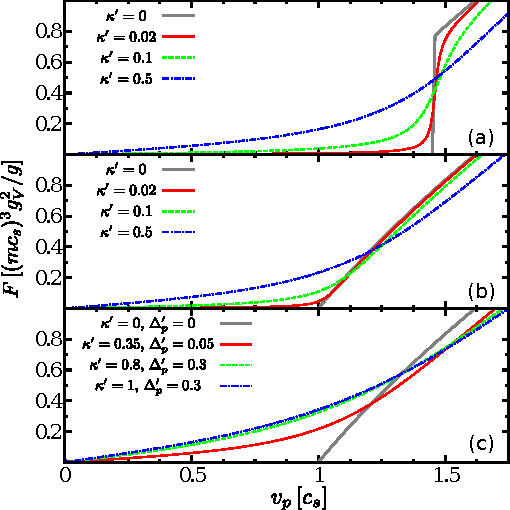
\includegraphics[width=0.6\linewidth]{dragspeed} % ~/ownCloud/documents/phd_projects/point_defect_1_fluid/paper/plots/dragspeed
\caption{
%
Drag force $F$ as a function of the fluid velocity
$v_p$ for different values of the pump detuning $\Delta_p$:
$\Delta_p=-0.3g|\Psi_0|^2$ (a), $\Delta_p=0$ (b), and $\Delta_p>0$
(c), and for different values of the polariton lifetime --- here, we
use the notation $\kappa' = \kappa/g|\psi_0|^2$ and $\Delta_p' =
\Delta/g|\psi_0|^2$.
%
}\label{fig:dragv}
\end{figure}
%
%
\begin{figure}[tb]\centering
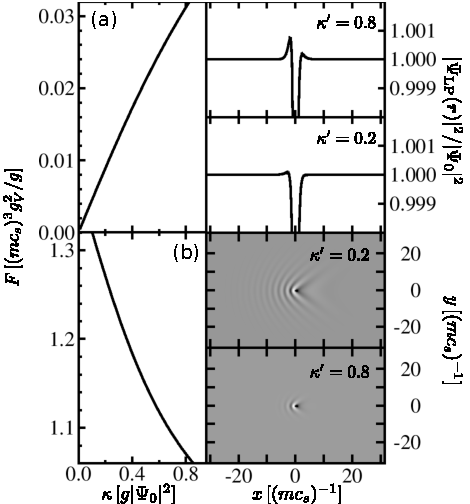
\includegraphics[width=0.6\linewidth]{dragkappa} % ~/ownCloud/documents/phd_projects/point_defect_1_fluid/paper/plots/kappa
\caption{
%
Drag force $F$ as a function of the inverse polariton
lifetime $\kappa'=\kappa/(g |\psi_0|^2)$ in the (a) subcritical regime
($v_p=0.2 c_s$) and (b) supercritical regime ($v_p=1.9 c_s$). In both
cases we have fixed $\Delta_p=-0.3g|\Psi_0|^2$ ($v^c \simeq 1.46 c_s$)
but these results are qualitatively similar for any other value of the
pump detuning. We plot in the insets the normalised real-space
wavefunction $|\psi_{LP}(\bm{r})|^2/|\psi_0|^2$ for two specific
values of $\kappa'=0.2$ and $\kappa'=0.8$.
%
}\label{fig:dragk}
\end{figure}
%


\section{Drag force}
\label{sec:drag}
%
The steady state response of the system to a static and weak defect
can be evaluated starting from Eq.~\eqref{eq:linre}:
%
\begin{equation*}
  \begin{pmatrix} \delta \psi_s(\bm{r}) \\ \delta
    \psi_s^*(\bm{r}) \end{pmatrix} =
  \hat{\mathcal{L}}^{-1} \begin{pmatrix} V(\bm{r}) e^{i \bm{k}_p
      \cdot \bm{r}} \psi_0 \\ -V(\bm{r}) e^{-i \bm{k}_p \cdot
      \bm{r}} \psi_0^{\star} \end{pmatrix} \; .
\end{equation*}
%
For a point-like defect, this can be written in momentum space as:
%
\begin{equation*}
  \delta \psi_s (\bm{k} + \bm{k}_p) = \frac{-g_V \psi_0
    (\varepsilon(\bm{k}) - \bm{k} \cdot \bm{v}_p +
    i\kappa)}{\varepsilon(\bm{k}) [\varepsilon(\bm{k}) +
      2g|\psi_0|^2] - (\bm{k} \cdot \bm{v}_p - i\kappa)^2} \; ,
\end{equation*}
%
while the other component $\delta \psi_s^* (\bm{k}_p - \bm{k})$
can be obtained by complex conjugation and by substituting $\bm{k}
\mapsto -\bm{k}$. The drag force exerted by the defect on the fluid
is given by~\cite{Astrakharchik_2004}:
%
\begin{equation}
  \bm{F} = - \int d\bm{r} |\psi_{LP}(\bm{r},t)|^2 \bm{\nabla}
  (V(\bm{r})) \; ,
\end{equation}
%
and, in the steady state linear response regime, we obtain:
%
\begin{multline}
  \bm{F} = g_V \int \frac{d\bm{k}}{(2\pi)^2} i\bm{k}
  \left[\psi_0^* \delta\psi_s (\bm{k} + \bm{k}_p) + \psi_0 \delta
    \psi_s^* (\bm{k}_p - \bm{k})\right]\\
%
  = 2g_V^2|\psi_0|^2 \int \frac{d\bm{k}}{(2\pi)^2} \frac{i\bm{k}
    \varepsilon(\bm{k})}{\omega^{+} (\bm{k})\omega^{-} (\bm{k})}
  \; .
    \label{eq:dragf}
\end{multline}
%
The drag is clearly oriented along the fluid velocity $\bm{v}_p$,
i.e., $\bm{F} = F \hat{\bm{v}}_p$. If $\kappa \to 0$, then the
integral in Eq.~\eqref{eq:dragf} is finite only if poles exist when
$\Re [\omega^{\pm} (\bm{k})] = 0$, i.e., when quasiparticles can be
excited, in agreement with the Landau criterion. For finite polariton
lifetimes, however, it is clear that the integral will always be
different from zero for $v_p>0$.
% Note that the only dependence on the polariton lifetime $\kappa$ is
%in the denominator of the integral in Eq.~\eqref{eq:dragf}.
We now analyse the behaviour of the drag force as a function of the
fluid velocity for the three ($\Delta_p = 0$, $\Delta_P > 0$, and
$\Delta_p < 0$) different spectra illustrated in the previous section.

For the \emph{linear} spectrum, at $\Delta_p=0$, in the equilibrium
limit, $\kappa \to 0$, we recover for the drag the known result of
weakly interacting Bose gases in two
dimensions~\cite{Astrakharchik_2004}:
%
\begin{equation}
  \frac{F}{(mc_s)^3 g_V^2/g}=\frac{(v_p/c_s)^2 - 1}{v_p/c_s}
  \Theta(v_p - c_s)\; ,
\label{eq:drag0}
\end{equation}
%
with a threshold-like behaviour at a critical fluid velocity equal to
the speed of sound $c_s$. This limiting result is plotted as a bold
gray line in the panels (b,c) of Fig.~\ref{fig:dragv}. For
$\Delta_p=0$ and finite lifetimes $\kappa$, we find a smooth crossover
from the subsonic to the supersonic regime, with the drag being closer
to the equilibrium threshold behaviour for decreasing $\kappa$ (see
Fig.~\ref{fig:dragv}(b)). A finite lifetime tends to increase the
value of the drag in the subsonic region $v_p \ll v^c$, giving place
to a residual drag force, similar to what was found in the numerical
simulations of Ref.~\cite{Cancellieri_2010}. Instead, in the supersonic
region $v_p \gg v^c$, the finite lifetime tends to decrease the value
of the drag. In the case of \emph{diffusive-like} spectra at
$\Delta_p>0$ the situation is qualitatively very similar to the
resonant case (see Fig.~\ref{fig:dragv}(c)), with the difference that
now, in order to have stable solutions, we can decrease the value of
the lifetime only by decreasing accordingly also the value of the pump
detuning $\Delta_p$. The crossover for both $\Delta_p = 0$ and
$\Delta_p > 0$ is also qualitatively very similar to the case of
non-resonantly pumped polaritons~\cite{Wouters_2010}, where the
spectrum of excitation is diffusive-like.

In the case of \emph{gapped} spectra, the situation is, however,
qualitatively different (see Fig.~\ref{fig:dragv}(a)). For infinitely
living polaritons, $\kappa \to 0$, the drag force can also be
evaluated analytically and its expression is similar to
Eq.~\eqref{eq:drag0}, but with a critical velocity larger than the
speed of sound, which expression is given in Eq.~\eqref{eq:criti}:
%
\begin{equation}
  \frac{F}{(mc_s)^3 g_V^2/g}=\frac{(v_p/c_s)^2 - 1}{v_p/c_s}
  \Theta(v_p - v^c)\; .
\end{equation}
%
Therefore now the drag experiences a jump for $v_p=v^c$, rather than a
continuous threshold as for the resonant case $\Delta_p=0$. As already
mentioned in the previous section, this discontinuous behaviour of the
drag for the gapped spectra is connected to the fact that, as soon as
quasiparticles can be excited by the defect at $v_p\ge v^c$,
Cherenkov-like waves can be immediately emitted in all directions,
rather than being restricted in a region outside the Mach cone as
before. For $\Delta_p=0$, the cone was gradually closing with
increasing  fluid velocity.

Both the increase of the value of the drag in the subcritical region
as a function of the polariton lifetime and the decrease in the
supercritical region, are behaviours common to all the types of
spectra. We plot the drag force as a function of $\kappa$ in
Fig.~\ref{fig:dragk}, for two values of the fluid velocity $v_p$ and a
specific value of the pump detuning $\Delta_p$, though we have checked
that the following results are generic. For $v_p < v^c$, we find that
the residual drag is a finite-lifetime effect only, and, in agreement
with the results of Ref.~\cite{Cancellieri_2010}, we find that, well
below the critical velocity, the drag force goes linearly to zero for
$\kappa \to 0$. In the resonant case $\Delta_p=0$, the slope of the
drag for $v_p \ll c_s$ can be evaluated analytically starting from the
expression~\eqref{eq:dragf}:
%
\begin{equation*}
    \frac{F}{(mc_s)^3 g_V^2/g} \mathop{\simeq}\limits_{\kappa \to 0} \frac{2 c_s}{\pi
      v_p} \left( \frac{1}{ \sqrt{1-(v_p/c_s)^2}} - 1 \right)
    \frac{\kappa}{g |\psi_0|^2} \; .
\end{equation*}
%
The residual drag in the subsonic regime is an effect of the
broadening of the quasi-particles energies: Even when the spectrum
real part does not allow any scattering against the defect (e.g., for
$\Delta_p \le 0$), the broadening produces some scattering close to
the defect. This results in a perturbation of the fluid around the
defect, asymmetric in the direction of the fluid velocity (see panel
(a) of Fig.~\ref{fig:dragk}), similar to what  was obtained in
Ref.~\cite{Cancellieri_2010}. Instead, in the supersonic regime, the
drag force is weaker in the non-equilibrium case with respect to the
equilibrium one. This is caused by the finite lifetime tending to
suppress the propagation of the Cherenkov waves away from the defect,
as shown in panel (b) of Fig.~\ref{fig:dragk}.




\section{Conclusions and discussion}
\label{sec:concl}
%
To conclude, we have analysed the linear response to a weak defect of
resonantly pumped polaritons in the pump-only state, and we have been
able to determine two different kinds of threshold like behaviours for
the drag force as a function of the fluid velocity. In the case of
either zero or positive pump detuning, one can continuously connect to
the case of equilibrium weakly interacting gases, where the drag
displays a continuous threshold with a critical velocity equal to the
speed of sound. However, for negative pump detuning, where the
spectrum of excitations is gapped, the drag shows a discontinuity with
a critical velocity larger than the speed of sound. In this sense, the
case of coherently driven microcavity polaritons in the pump-only
configuration displays a richer phenomenology than the case of
polariton superfluids non resonantly pumped. It would be interesting
to perform a similar analysis in the case of polaritons in the optical
parametric oscillator regime, where polaritons are parametrically
scattered from the pump state to the signal and idler states. Here,
the spectrum of excitations has been already determined in
Ref.~\cite{Wouters_2007}, however it is far from clear what are the
conditions for subcritical, superfluid, behaviour in a fluid
characterised by three distinct currents, and how the link between
signal and idler imposed by the parametric scattering influences the
scattering of both fluids against a defect.


\begin{subappendices}
\section{Gross-Pitaevskii equation for the LP field}
\label{app:full}
%
% TODO: make link to formulas in Chapter 3
If one starts from a descriptions of polaritons in terms of separate
exciton and cavity photon fields, a rotation into the lower and upper
polariton basis, followed by neglecting the occupancy of the upper
polariton branch, results in the following Gross-Pitaevskii equation
for the LP field in momentum space
$\psi_{LP}(\bm{r},t) = \sum_{\bm{k}} e^{i\bm{k}\cdot \bm{r}}
\psi_{LP,\bm{k}} (t)$~\cite{Ciuti_2003}:
%
\begin{multline}
  i\partial_t \psi_{LP,\bm{k}} = f_p e^{-i\omega_p t}
  \delta_{\bm{k},\bm{k}_p} + \left[\omega_{LP} (k) - i\kappa
    (k)\right]\psi_{LP,\bm{k}} +\\
%
  \sum_{\bm{k}_1, \bm{k}_2} g_{\bm{k}, \bm{k}_1, \bm{k}_2}
  \psi^*_{LP,\bm{k}_1 + \bm{k}_2-\bm{k}} \psi_{LP,\bm{k}_1}
  \psi_{LP,\bm{k}_2} +\\ s_k \sum_{\bm{k}_1} V_{\bm{k} -
    \bm{k}_1} \psi_{LP,\bm{k}_1} s_{k_1}\; ,
\end{multline}
%
where $\kappa(k)=\kappa_X c^2_k + \kappa_C s^2_k$ is the effective LP
decay rate,
%
\begin{equation}
  g_{\bm{k}, \bm{k}_1, \bm{k}_2}=g_X c_{k}c_{|\bm{k}_1 + \bm{k}_2-\bm{k}|} c_{k_1} c_{k_2}
\end{equation}
%
is the interaction strength, and where
$V(\bm{r}) = \sum_{\bm{k}} e^{i\bm{k}\cdot \bm{r}} V_{\bm{k}}$.

In these expressions, the coefficients
%
\begin{equation}
  c^2_{k}, s^2_{k} = \frac{1}{2} \left(1 \pm \frac{\omega_C(k) -
    \omega_X^0}{\sqrt{(\omega_C(k) - \omega_X^0)^2 +
      \Omega_R^2}}\right)
\end{equation}
%
are the Hopfield coefficients used to diagonalise the free polariton
Hamiltonian. We want here to justify the simplified description done
in Eq.~\eqref{eq:basic}. If we follow the linear response expansion as
in~\eqref{eq:mfield}, the operator $\hat{\mathcal{L}}$ in momentum
space analogous to~\eqref{eq:opell} reads as:

%
\begin{equation}
  \mathcal{L}_{\bm{k},\bm{k}_p} = \begin{pmatrix}
    \widetilde{\omega_{LP}} (\delta \bm{k}+\bm{k}_p) - i
    \kappa(\delta \bm{k}+\bm{k}_p) & g_X c_{k_p}^2 c_{\delta
      \bm{k}+\bm{k}_p} c_{\delta \bm{k}-\bm{k}_p} \psi_0^2
    \\ - g_X c_{k_p}^2 c_{\delta \bm{k}+\bm{k}_p} c_{\delta
      \bm{k}-\bm{k}_p}{\psi_0^{\star}}^2 & -
    \widetilde{\omega_{LP}}(\delta \bm{k}-\bm{k}_p) -
    i\kappa(\delta \bm{k}-\bm{k}_p) \end{pmatrix}\; ,
\label{eq:opel2}
\end{equation}
%

where now $\widetilde{\omega_{LP}} (\delta \bm{k} \pm\bm{k}_p) =
\omega_{LP} (\delta \bm{k} \pm\bm{k}_p) -\omega_p + 2 g_X
c_{k_p}^2 c_{\delta \bm{k} \pm \bm{k}_p}^2 |\psi_0|^2$. It is easy
to show that the eigenvalues of this operator coincide with our
approximated expressions~\eqref{eq:spect} in the limit of $\delta k
\ll k_p$, when $c_{\delta \bm{k} \pm \bm{k}_p}^2 \simeq
c_{k_p}^2$, $s_{\delta \bm{k} \pm \bm{k}_p}^2 \simeq s_{k_p}^2$
and when we can simply rename $g=g_X c_{k_p}^4$ and $\kappa =
\kappa(k_p)$. It is interesting to note that, even if we would retain
the linear terms in $\bm{k}_p \cdot \delta \bm{k}$ in the
expansion of $c_{\delta \bm{k} \pm \bm{k}_p}^2$, this would result
in a renormalisation of the fluid velocity $\bm{v}_p$ in the
expression~\eqref{eq:spect} which takes into account the blue-shift of
the lower polariton dispersion due to the interaction.

\end{subappendices}

% TODO: cite Larr__2012 (1D case)
% TODO: include residual drag figure from Cancellieri_2010
% TODO: cite Van_Regemortel_2014 (negative drag)
% TODO: Amo_2009 -- include pic; fig. 2&20 QFL

%%% Local Variables:
%%% mode: latex
%%% TeX-master: "../thesis_berceanu"
%%% End:



\backmatter

% Bibliography should be called "References":
\bibliographystyle{thesis}
\renewcommand{\bibname}{References}
\bibliography{index}

\addcontentsline{toc}{part}{References}

\chapter*{Summary}
\markboth{Summary}{}
\addcontentsline{toc}{part}{Summary}

Lorem ipsum dolor sit amet, consectetuer adipiscing elit.  Donec hendrerit tempor tellus.  Donec pretium posuere tellus.  Proin quam nisl, tincidunt et, mattis eget, convallis nec, purus.  Cum sociis natoque penatibus et magnis dis parturient montes, nascetur ridiculus mus.  Nulla posuere.  Donec vitae dolor.  Nullam tristique diam non turpis.  Cras placerat accumsan nulla.  Nullam rutrum.  Nam vestibulum accumsan nisl.

Pellentesque dapibus suscipit ligula.  Donec posuere augue in quam.  Etiam vel tortor sodales tellus ultricies commodo.  Suspendisse potenti.  Aenean in sem ac leo mollis blandit.  Donec neque quam, dignissim in, mollis nec, sagittis eu, wisi.  Phasellus lacus.  Etiam laoreet quam sed arcu.  Phasellus at dui in ligula mollis ultricies.  Integer placerat tristique nisl.  Praesent augue.  Fusce commodo.  Vestibulum convallis, lorem a tempus semper, dui dui euismod elit, vitae placerat urna tortor vitae lacus.  Nullam libero mauris, consequat quis, varius et, dictum id, arcu.  Mauris mollis tincidunt felis.  Aliquam feugiat tellus ut neque.  Nulla facilisis, risus a rhoncus fermentum, tellus tellus lacinia purus, et dictum nunc justo sit amet elit.

Lorem ipsum dolor sit amet, consectetuer adipiscing elit.  Donec hendrerit tempor tellus.  Donec pretium posuere tellus.  Proin quam nisl, tincidunt et, mattis eget, convallis nec, purus.  Cum sociis natoque penatibus et magnis dis parturient montes, nascetur ridiculus mus.  Nulla posuere.  Donec vitae dolor.  Nullam tristique diam non turpis.  Cras placerat accumsan nulla.  Nullam rutrum.  Nam vestibulum accumsan nisl.



\chapter*{Resumen}
\markboth{Resumen}{}
\addcontentsline{toc}{part}{Resumen}
\selectlanguage{spanish}

Pellentesque dapibus suscipit ligula.  Donec posuere augue in quam.  Etiam vel tortor sodales tellus ultricies commodo.  Suspendisse potenti.  Aenean in sem ac leo mollis blandit.  Donec neque quam, dignissim in, mollis nec, sagittis eu, wisi.  Phasellus lacus.  Etiam laoreet quam sed arcu.  Phasellus at dui in ligula mollis ultricies.  Integer placerat tristique nisl.  Praesent augue.  Fusce commodo.  Vestibulum convallis, lorem a tempus semper, dui dui euismod elit, vitae placerat urna tortor vitae lacus.  Nullam libero mauris, consequat quis, varius et, dictum id, arcu.  Mauris mollis tincidunt felis.  Aliquam feugiat tellus ut neque.  Nulla facilisis, risus a rhoncus fermentum, tellus tellus lacinia purus, et dictum nunc justo sit amet elit.

Lorem ipsum dolor sit amet, consectetuer adipiscing elit.  Donec hendrerit tempor tellus.  Donec pretium posuere tellus.  Proin quam nisl, tincidunt et, mattis eget, convallis nec, purus.  Cum sociis natoque penatibus et magnis dis parturient montes, nascetur ridiculus mus.  Nulla posuere.  Donec vitae dolor.  Nullam tristique diam non turpis.  Cras placerat accumsan nulla.  Nullam rutrum.  Nam vestibulum accumsan nisl.

Aliquam erat volutpat.  Nunc eleifend leo vitae magna.  In id erat non orci commodo lobortis.  Proin neque massa, cursus ut, gravida ut, lobortis eget, lacus.  Sed diam.  Praesent fermentum tempor tellus.  Nullam tempus.  Mauris ac felis vel velit tristique imperdiet.  Donec at pede.  Etiam vel neque nec dui dignissim bibendum.  Vivamus id enim.  Phasellus neque orci, porta a, aliquet quis, semper a, massa.  Phasellus purus.  Pellentesque tristique imperdiet tortor.  Nam euismod tellus id erat.




\end{document}

\newpage

%%% Local Variables:
%%% mode: latex
%%% TeX-master: t
%%% End:
